\documentclass[conference]{IEEEtran}
\usepackage[utf8]{inputenc}
\usepackage[T1]{fontenc}
\usepackage{hyperref}
\usepackage[backend=biber, style=ieee]{biblatex}
\usepackage{amssymb}
\usepackage{amsmath}
\usepackage{float}
\usepackage{booktabs}
\usepackage{csquotes}
\usepackage{microtype}
\usepackage{array}
\usepackage{graphicx}
\usepackage{tikz}
\usetikzlibrary{arrows.meta,calc}
\usepackage{placeins}
\addbibresource{ref.bib}

\title{State of the art about network traffic generation for dataset creation}

\author{
\IEEEauthorblockN{Evan JOASSON \\ July 2026}
}

\begin{document}

\maketitle

\begin{abstract}
Machine learning-based intrusion detection systems (IDS) require
large-scale, diverse, and correctly labeled network traffic datasets,
yet such data remains scarce. Real-world captures raise privacy
concerns, and the benchmark datasets that dominate the literature are
variously outdated, mislabeled, or unrepresentative of real traffic.
This survey reviews the state of the art in network traffic generation
as a potential remedy to this ``data problem,'' organizing existing
tools into four families --- traffic replay, packet crafting, synthetic
and injection-based approaches, and containerized environments --- and
comparing their trade-offs between realism, flexibility, and
reproducibility. Contrasting the two most mature approaches, ID2T and
ConCap, we show that neither reconciles topological realism, privacy,
and dataset quality at once. One preserves the fingerprint of a real
network but still depends on a real capture, while the other removes
that dependency at the cost of a flat, infrastructure-free network. We
conclude that generating fresh, realistic, and correctly labeled
datasets remains an open challenge for the NIDS research.
\end{abstract}

\section{Introduction}

\subsection{Global Context}

Network infrastructures have become the backbone of modern organizations,
and with that comes an ever-growing attack surface. Over the past decade,
the volume and sophistication of cyber-threats have increased to a point
where manual monitoring is simply no longer viable. Intrusion Detection
Systems (IDS) have emerged as a cornerstone of network defense, sitting
between raw traffic and human analysts (SOC Team) to flag anomalous or malicious
behavior \cite{sharafaldin2018}.

For a long time, signature-based IDS dominated the field, they work well
against known attacks but fail completely the moment an attacker slightly
modifies their approach. This fundamental limitation has pushed the research
community toward machine learning (ML), which offers the ability to generalize
and detect threats that were never explicitly programmed \cite{survey2026}.
The catch, however, is that ML models are only as good as the data they
are trained on.

\subsection{Problem Statement}

Building a reliable ML-based IDS demands large-scale, diverse, and
accurately labeled network traffic datasets. In practice, this is
surprisingly hard to come by. Real-world traffic captured from production
networks raises immediate privacy concerns, packet payloads may carry
sensitive user data, and operators are rarely willing --- or legally
permitted --- to share such captures publicly \cite{ring2019}. Even when
data can be collected, labeling it is a labor-intensive process that
requires domain expertise for every single flow.

The consequence is a research landscape that has long relied on a
handful of aging benchmark datasets. DARPA 1998, KDD99, and even
CICIDS2017 \cite{sharafaldin2018} are now considered outdated by many
in the community: they reflect network conditions, attack patterns, and
protocol distributions from a different era. As shown in \cite{id2t2021},
most publicly available datasets carry inherent negative qualities ---
lack of traffic diversity, unrealistic background traffic, absent or
incorrect labels --- that silently bias the systems trained and evaluated
on them. Training on such data leads to models that perform well in
controlled benchmarks yet struggle in real deployments.

Apart from being outdated, the datasets generated by test benches face a range 
of problems specific to them. Lab environments tend to oversimplify network conditions,
a handful of machines generating scripted traffic cannot reproduce
the behavioral diversity of thousands of real users \cite{ring2019}.
Attack traffic injected in these settings is often inefficient or
misconfigured, and fails to match what the same attack looks like
in the wild \cite{survey2025}.


\section{Related Work}
\subsection{Existing Traffic Generation Tools}

Network traffic generators can be broadly divided into four families,
each with distinct trade-offs when it comes to producing datasets
suitable for IDS training \cite{adeleke2022}. Figure~\ref{fig:taxonomy}
gives an overview of this taxonomy before each family is discussed
in detail below.

\begin{figure*}[!t]
\centering
\resizebox{\textwidth}{!}{%
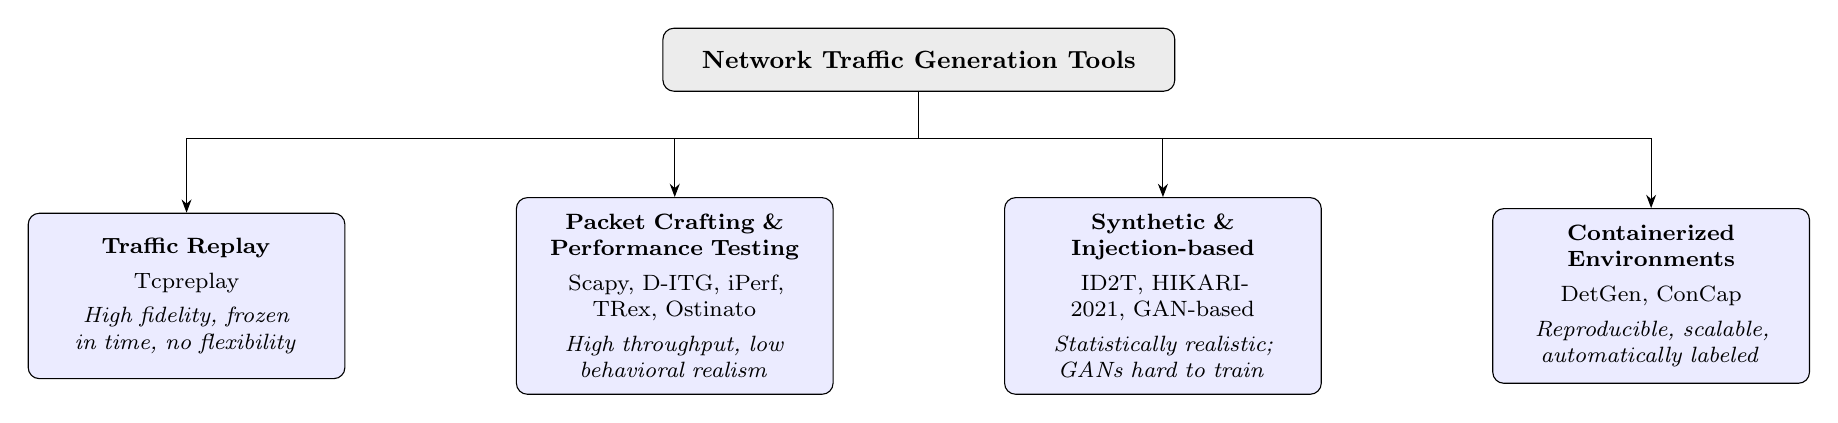
\begin{tikzpicture}[
  every node/.style={draw, rounded corners, align=center, font=\footnotesize, inner sep=6pt},
  root/.style={fill=gray!15, minimum width=6.5cm, minimum height=0.8cm, font=\small\bfseries},
  family/.style={fill=blue!8, text width=3.6cm, minimum height=2.1cm},
  >=Stealth
]
\node[root] (root) at (0,0) {Network Traffic Generation Tools};

\node[family] (replay)    at (-9.3,-3.0) {\textbf{Traffic Replay}\\[3pt] Tcpreplay\\[3pt] \textit{High fidelity, frozen in time, no flexibility}};
\node[family] (crafting)  at (-3.1,-3.0) {\textbf{Packet Crafting \& Performance Testing}\\[3pt] Scapy, D-ITG, iPerf, TRex, Ostinato\\[3pt] \textit{High throughput, low behavioral realism}};
\node[family] (synthetic) at (3.1,-3.0)  {\textbf{Synthetic \& Injection-based}\\[3pt] ID2T, HIKARI-2021, GAN-based\\[3pt] \textit{Statistically realistic; GANs hard to train}};
\node[family] (container) at (9.3,-3.0)  {\textbf{Containerized Environments}\\[3pt] DetGen, ConCap\\[3pt] \textit{Reproducible, scalable, automatically labeled}};

\draw (root.south) -- (0,-1.0);
\draw (-9.3,-1.0) -- (9.3,-1.0);
\draw[->] (-9.3,-1.0) -- (replay.north);
\draw[->] (-3.1,-1.0) -- (crafting.north);
\draw[->] (3.1,-1.0)  -- (synthetic.north);
\draw[->] (9.3,-1.0)  -- (container.north);
\end{tikzpicture}%
}
\caption{Taxonomy of network traffic generation tool families discussed in this survey.}
\label{fig:taxonomy}
\end{figure*}

The oldest and simplest approach is \textbf{traffic replay}. Tools
such as Tcpreplay read a pre-recorded PCAP file and retransmit its
packets onto a live interface. While this preserves the statistical
properties of a real capture, it offers no flexibility: the traffic
is frozen in time, reflects a specific network environment, and
carries no new attack scenarios. Replaying complex multi-party
attacks is particularly problematic, as most replay tools are
stateless and cannot reconstruct the two-sided nature of a
connection \cite{survey2025}.

A second family groups \textbf{packet crafting and performance testing}
tools. Scapy allows users to build and send arbitrary packets through
a Python scripting interface, offering fine-grained control over every
header field. D-ITG and iPerf focus on generating high-throughput flows
to stress-test network links, while Cisco TRex and Ostinato target
commercial network equipment validation. A quantitative comparison of
TRex, Ostinato and Genesids conducted by \textcite{koay2021} showed
that while these tools can reach high packet rates, their traffic lacks
behavioral realism: payloads are either absent or randomly generated,
and the resulting flows bear little resemblance to genuine application
traffic. For IDS training, where the subtlety of an attack pattern
matters as much as its volume, this is a fundamental limitation.

More recently, \textbf{synthetic and injection-based} generators have
emerged as a promising middle ground. \textcite{id2t2021} take a
different stance. Rather than generating traffic from scratch, they
inject synthetic attacks directly into a real background capture,
carefully mimicking the statistical properties of the surrounding
traffic to avoid leaving detectable artifacts. Similarly,
\textcite{hikari2021} proposed a methodology for generating encrypted
synthetic attack traffic in a real-world network environment, producing
the HIKARI-2021 dataset, which addressed a gap that most existing
datasets ignored, the prevalence of TLS-encrypted attack vectors. On
the generative side, approaches based on Generative Adversarial Networks
(GANs) --- such as the flow-based generator proposed by
\textcite{ring2019gan} --- attempt to learn the underlying distribution
of real traffic and sample new flows from it. Despite encouraging
results, GAN-based methods remain difficult to train and often struggle
to capture the temporal dependencies and protocol constraints that
characterize realistic network traffic \cite{adeleke2022}.

A fourth and more recent family leverages \textbf{containerized
environments} to generate labeled network traffic in a lightweight,
reproducible manner. The key insight behind these approaches is that
containers faithfully replicate the network behavior of physical
machines, while providing complete control over the attacker and target
hosts without requiring a dedicated physical testbed. \textcite{detgen2021}
were among the first to explore this direction with DetGen, which uses
Docker containers to generate traffic for ML-based NIDS. Building on
this idea, \textcite{concap2026} proposed ConCap (Container Capture),
which addresses several limitations of its predecessors. ConCap relies
on Kubernetes to orchestrate isolated containerized environments and
supports concurrent execution of multiple attack scenarios, fine-grained
control over network conditions (bandwidth, latency, packet loss), and
automatic NetFlow extraction and labeling. A key advantage of ConCap
is its scenario-based configuration: a single YAML file fully describes
an experiment, enabling other researchers to reproduce the exact same
traffic without sharing potentially large dataset files. Empirical
validation showed that ConCap's generated traffic is functionally
equivalent to that of physical bare-metal setups from a machine
learning standpoint \cite{concap2026}.

Across all four families, a common thread emerges: existing tools
were primarily designed for performance testing, network emulation,
or isolated attack reproduction, not for the controlled and scalable
production of diverse, labeled security datasets. Table~\ref{tab:tools}
summarizes the trade-offs of each family along three axes: the
realism of the traffic they produce, the degree of control and
flexibility they offer, and their main limitation for dataset
generation.

\begin{table*}[!t]
  \centering
  \caption{Comparison of the four families of network traffic
           generation tools.}
  \label{tab:tools}
  \begin{tabular}{lp{3.2cm}ccp{5.6cm}}
    \toprule
    \textbf{Family} & \textbf{Representative Tools} & \textbf{Realism} &
    \textbf{Control / Flexibility} & \textbf{Main Limitation} \\
    \midrule
    Traffic Replay &
      Tcpreplay &
      High &
      Low &
      Frozen in time; stateless, cannot reconstruct multi-party attacks \\
    Packet Crafting \& Perf.\ Testing &
      Scapy, D-ITG, iPerf, TRex, Ostinato &
      Low &
      High &
      Payloads absent or random; lacks behavioral realism \\
    Synthetic \& Injection-based &
      ID2T, HIKARI-2021, GAN-based generators &
      High &
      Medium &
      GAN-based methods hard to train; depend on background capture \\
    Containerized Environments &
      DetGen, ConCap &
      High &
      High &
      Requires container/orchestration infrastructure (Docker, Kubernetes) \\
    \bottomrule
  \end{tabular}
\end{table*}

\subsection{IDS Datasets and Their Limitations}

Publicly available labeled datasets are the foundation on which
ML-based IDS research is built. Without them, it is impossible
to train classifiers, reproduce experiments, or compare methods
across papers. Yet, as \textcite{ring2019} documented in a survey
of over 30 datasets, the landscape is dominated by a small number
of aging benchmarks whose limitations are well known but routinely
overlooked.

\subsubsection{Benchmark Dataset Landscape}

Table~\ref{tab:datasets} summarizes the four datasets most
frequently encountered in the NIDS literature. Together, they
cover a decade of dataset construction efforts, yet each carries
structural problems that limit its usefulness for training
modern ML-based detectors.

\begin{table*}[!t]
  \centering
  \caption{Overview of major benchmark NIDS datasets and their
           known limitations.}
  \label{tab:datasets}
  \begin{tabular}{lcccp{9cm}}
    \toprule
    \textbf{Dataset} & \textbf{Year} & \textbf{Encrypted} &
    \textbf{Labeled} & \textbf{Known Issues} \\
    \midrule
    NSL-KDD     & 2009 & \texttimes & \checkmark &
      Outdated attacks, statistical artifacts, simulated network \\
    UNSW-NB15   & 2015 & \texttimes & \checkmark &
      Class imbalance, class overlap, testbed conditions \\
    CICIDS2017  & 2017 & \texttimes & \checkmark &
      Labeling errors, CICFlowMeter bugs, unrealistic background traffic \\
    TON-IoT     & 2020 & Partial    & \checkmark &
      Severe class imbalance (96\% attacks), IoT-specific, poor generalization \\
    \bottomrule
  \end{tabular}
\end{table*}

\textbf{NSL-KDD} was introduced in 2009 to address the redundancy
issues of its predecessor KDD99, but the underlying network
conditions remain those of a 1998 military testbed. Structural
artifacts --- TTL values and source IP addresses that differ
systematically between benign and attack traffic --- allow naive
classifiers to reach near-perfect accuracy without learning
anything meaningful about actual network behavior \cite{survey2025}.
Despite this, the dataset continued to appear in the majority of
NIDS publications well into the 2020s.

\textbf{UNSW-NB15} \cite{moustafa2015} was generated at the
Australian Centre for Cyber Security using the IXIA PerfectStorm
tool. While it introduced a broader range of modern attack types,
it suffers from significant class imbalance and class overlap:
benign and attack samples share feature regions that are difficult
to separate, and certain attack categories are severely
underrepresented \cite{zoghi2024}. These two issues compound
each other, making any classifier trained on raw UNSW-NB15 prone
to boundary misclassification.

\textbf{CICIDS2017} \cite{sharafaldin2018} quickly became the
de facto benchmark of the field, accumulating over 4200 citations
by late 2024 \cite{concap2026}. However, \textcite{engelen2021}
revealed systematic labeling errors rooted in a faulty
implementation of CICFlowMeter: TCP flows were incorrectly
terminated, RST packets were ignored, and the resulting mislabeled
samples silently skew any classifier trained on them. These
findings were later extended and confirmed independently, leading
to the release of corrected versions of both CICIDS2017 and its
successor CSE-CIC-IDS2018.

\textbf{TON-IoT} \cite{alsaedi2020} addresses the growing
importance of IoT network security and covers nine attack
categories across a heterogeneous testbed. Its most glaring
problem, however, is a severe class imbalance: attack traffic
accounts for 96.44\% of all records, leaving only 3.56\% for
benign flows \cite{dinh2026}. A model trained on such a
distribution learns to classify almost everything as malicious
--- a behavior that would be operationally catastrophic in a
real deployment.

\subsubsection{Recurring Design Flaws}

Beyond the specificities of each dataset, \textcite{flood2024}
identified six design flaws that recur systematically across
the benchmarks used in NIDS research: limited feature diversity,
high feature interdependence, ambiguous ground truth, collapse
of traffic distributions, artificially generated diversity, and
labeling inaccuracies. This work, awarded Best Paper at IEEE
EuroS\&P 2024, raises serious doubts about the validity of
results reported across a large portion of the existing
literature.

\textbf{Class imbalance} is perhaps the most common of these
vulnerabilities. In real networks, attacks are rare events, a classifier
that labels every flow as benign would achieve accuracy above
99\% on most captures, yet detect nothing. Benchmark datasets
amplify this problem in both directions --- TON-IoT skews
toward attacks while UNSW-NB15 is predominantly benign ---
forcing researchers to resort to artificial resampling techniques
that may themselves introduce new biases \cite{dinh2026}.

\textbf{Non-representativeness} is a subtler but equally serious
problem. \textcite{layeghy2022} directly compared the
statistical properties of benign traffic in CICIDS2017, UNSW-NB15,
and TON-IoT against two real-world network captures. The
differences were substantial: packet size distributions, inter-arrival
times, and protocol ratios all diverge significantly between
testbed-generated and real traffic. Their conclusion is direct,
high accuracy on synthetic benchmark datasets does not guarantee
performance in real deployments.

\textbf{Feature leakage} compounds the representativeness problem.
In several widely used datasets, certain features --- such as
source or destination IP addresses, port numbers assigned
specifically to the attack tool, or timestamps that perfectly
separate attack days from benign days --- act as unintended
shortcut cues. A model that learns these spurious correlations
will show inflated performance metrics on held-out test sets
drawn from the same dataset, while failing immediately on any
other network \cite{flood2024}.

Finally, most datasets are \textbf{blind to encrypted traffic}.
As \textcite{hikari2021} pointed out, the vast majority of modern
attacks are delivered over HTTPS and TLS, yet NSL-KDD, UNSW-NB15,
and CICIDS2017 contain little to no such traffic. A detector
trained on cleartext flows is structurally unable to handle the
dominant attack vector of the modern Internet.

Taken together, these limitations paint a consistent picture:
the datasets available to the community are either too old,
incorrectly labeled, statistically unrepresentative, or blind
to encrypted traffic. Generating fresh, correctly labeled,
and realistic datasets from scratch remains an open challenge.


\section{Discussion}

Among the four families surveyed, traffic replay and packet crafting
tools can be set aside quickly. The first is frozen in time and
does not allow for the consideration of new attack scenarios, whilst the second prioritises
throughput at the expense of realistic behaviour in terms of the payload. 
The remaining two families --- synthetic/injection-based and containerized 
approaches --- represent the current state of the art, and \textcite{id2t2021} and
\textcite{concap2026} are arguably their most mature instances, ID2T
and ConCap, respectively. Confronting these two tools is instructive,
as they embody two fundamentally different philosophies for the same
goal.

\begin{figure*}[!t]
\centering
\resizebox{\textwidth}{!}{%
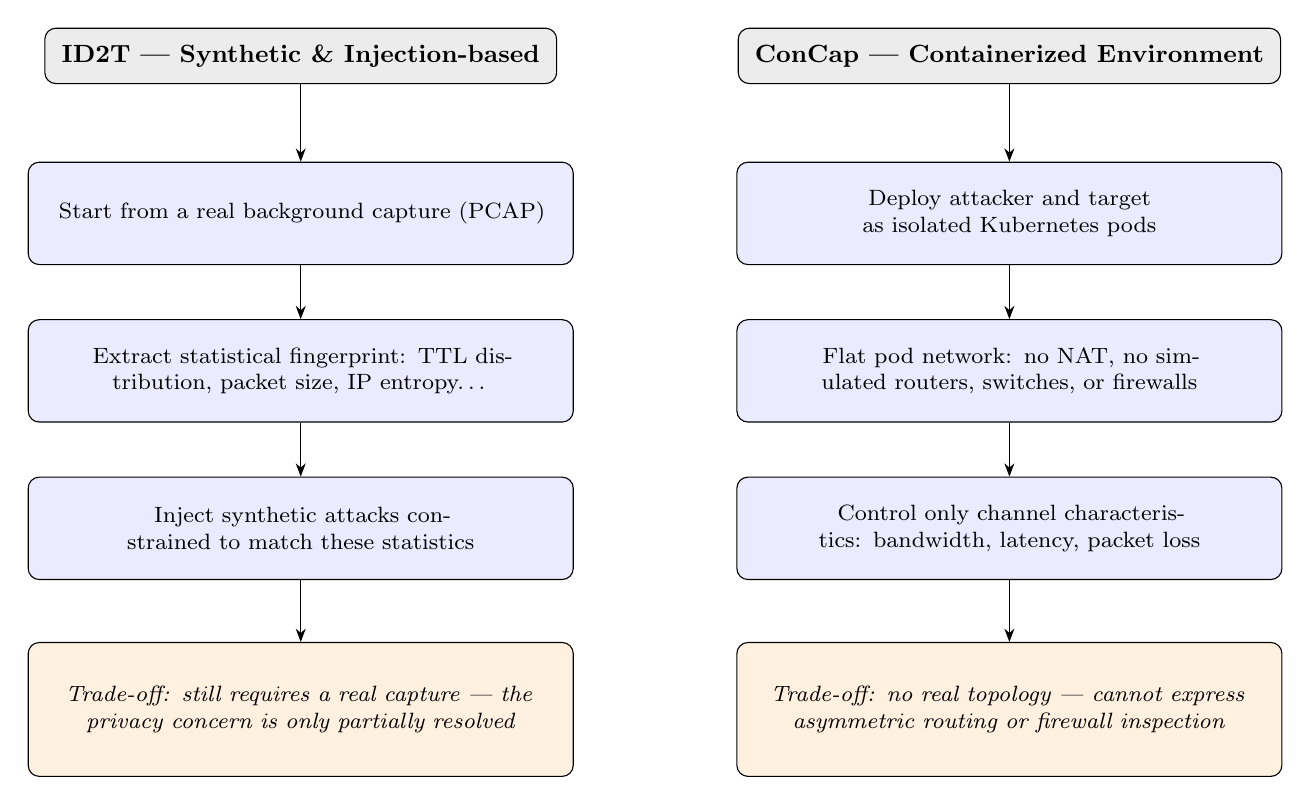
\begin{tikzpicture}[
  every node/.style={draw, rounded corners, align=center, font=\footnotesize, inner sep=6pt},
  header/.style={fill=gray!15, minimum width=6.5cm, font=\small\bfseries},
  procbox/.style={fill=blue!8, text width=6.5cm, minimum height=1.3cm},
  tradeoff/.style={fill=orange!12, text width=6.5cm, minimum height=1.7cm, font=\footnotesize\itshape},
  >=Stealth
]

\node[header] (id2t-h) at (-4.5,0) {ID2T --- Synthetic \& Injection-based};
\node[procbox]   (id2t-1) at (-4.5,-2.0) {Start from a real background capture (PCAP)};
\node[procbox]   (id2t-2) at (-4.5,-4.0) {Extract statistical fingerprint: TTL distribution, packet size, IP entropy\ldots};
\node[procbox]   (id2t-3) at (-4.5,-6.0) {Inject synthetic attacks constrained to match these statistics};
\node[tradeoff] (id2t-t) at (-4.5,-8.3) {Trade-off: still requires a real capture --- the privacy concern is only partially resolved};

\draw[->] (id2t-h) -- (id2t-1);
\draw[->] (id2t-1) -- (id2t-2);
\draw[->] (id2t-2) -- (id2t-3);
\draw[->] (id2t-3) -- (id2t-t);

\node[header] (cc-h) at (4.5,0) {ConCap --- Containerized Environment};
\node[procbox]   (cc-1) at (4.5,-2.0) {Deploy attacker and target as isolated Kubernetes pods};
\node[procbox]   (cc-2) at (4.5,-4.0) {Flat pod network: no NAT, no simulated routers, switches, or firewalls};
\node[procbox]   (cc-3) at (4.5,-6.0) {Control only channel characteristics: bandwidth, latency, packet loss};
\node[tradeoff] (cc-t) at (4.5,-8.3) {Trade-off: no real topology --- cannot express asymmetric routing or firewall inspection};

\draw[->] (cc-h) -- (cc-1);
\draw[->] (cc-1) -- (cc-2);
\draw[->] (cc-2) -- (cc-3);
\draw[->] (cc-3) -- (cc-t);

\end{tikzpicture}%
}
\caption{ID2T vs. ConCap: two opposing philosophies for generating
IDS traffic.}
\label{fig:id2t-vs-concap}
\end{figure*}

ID2T injects synthetic attack packets into a pre-existing, real
background capture. Because that background traffic already traversed
whatever real infrastructure the original network relied on (routers,
switches, firewalls), it inherently carries the statistical fingerprint
of that infrastructure --- most notably in properties such as TTL
distribution, which reflects the number of hops a packet crossed.
ID2T does not simulate this infrastructure at injection time, rather,
it computes statistics from the background capture and constrains the
injected packets to reproduce them, so that the synthetic traffic
remains statistically indistinguishable from traffic that genuinely
crossed the same network path \cite{id2t2021}. ConCap, by contrast,
generates all of its traffic from scratch inside a Kubernetes cluster,
where the attacker and target hosts run as separate pods. The
Kubernetes pod network is, by design, flat. Every pod can reach every
other pod directly, without NAT, and ConCap's scenario files only let
a researcher tune the channel between attacker and target ---
bandwidth, latency, packet loss --- not intermediate routing,
switching, or filtering behavior \cite{concap2026}. In other words,
ID2T inherits a real network's topology signature through its
background traffic without needing to simulate it, whereas ConCap
sidesteps the issue entirely by generating traffic on a
topology-free, point-to-point channel.

This opposition has a direct bearing on the privacy problem raised in
the Introduction. ID2T still requires a real background capture,
meaning the confidentiality concerns it was meant to help avoid are
only partially addressed. ConCap requires no real capture at all,
eliminating that dependency, but its flat, infrastructure-free
network also means it cannot express behaviors that depend on genuine
topology, such as traffic shaped by asymmetric routing, stateful
firewall inspection, or multi-hop latency accumulation. Neither tool,
therefore, offers a complete answer, one sacrifices privacy for
topological realism, the other sacrifices topological realism for
reproducibility and privacy.

This trade-off also leaves several limitations identified in the
dataset landscape only partially addressed. Neither ID2T nor ConCap
explicitly tackles class imbalance or feature leakage, both leave
label proportions and feature distributions to the researcher's
configuration rather than enforcing safeguards against them.
Non-representativeness is the one flaw for which ConCap offers a
concrete, if partial, answer: \textcite{concap2026} report packet-
and NetFlow-level comparisons against a bare-metal environment, as
well as an evaluation on a real ``smart-home'' network, showing that
ML classifiers trained on one environment generalize almost perfectly
to the other. This directly speaks to the representativeness gap
highlighted by \textcite{layeghy2022} --- but only for the handful of
network activities tested (port scans, brute-forcing, denial-of-service);
whether this equivalence holds at the scale and behavioral diversity
of a full enterprise network, the very diversity Layeghy and Portmann
measured across benign traffic, remains untested. Encrypted traffic is
only partially covered --- HIKARI-2021 fills that specific gap
\cite{hikari2021}, but neither ID2T nor ConCap is validated against
TLS-specific traffic. The traffic generation literature and the
dataset limitation literature therefore remain only loosely connected.
The tools most capable of producing fresh, labeled data are not
evaluated against the very criteria that make existing benchmark
datasets unreliable, leaving open whether a next-generation dataset
built with these tools would, in fact, make it possible to avoid the weaknesses 
mentioned above.


\section{Conclusion}

This survey provided a comprehensive review of network traffic generation methods 
designed to overcome the persistent ``data problem'' in ML-based NIDS research. 
By establishing a taxonomy across four distinct tool families --- traffic replay, 
packet crafting, synthetic injection, and containerized environments --- we categorized 
their operational trade-offs across realism, flexibility, and reproducibility. 
Furthermore, an analysis of widely used benchmark datasets highlighted structural 
vulnerabilities, including labeling errors, feature leakage, class imbalance, and 
a widespread blindness to encrypted traffic, which continue to compromise model evaluation.

Confronting the two most mature traffic generation approaches, ID2T
and ConCap, revealed that no single tool currently reconciles
topological realism, privacy, and dataset-quality guarantees at once:
one preserves the fingerprint of a real network but still depends on
a real background capture, while the other removes that dependency
at the cost of a flat, infrastructure-free network. Neither tool
explicitly addresses class imbalance or feature leakage, and the
empirical evidence available for representativeness remains limited
to a narrow set of network activities. Taken together, these findings
confirm that generating fresh, correctly labeled, and realistic
network traffic datasets remains an open challenge for the NIDS
research.

Consequently, closing the gap between generated traffic and real-world network 
deployments remains an open challenge. To address this, future research 
should explore hybrid approaches that integrate virtual network components 
(e.g., switches, firewalls, and asymmetric routing) directly into containerized 
environments. Additionally, future traffic generators must include automated 
validation checks to systematically prevent feature leakage and class imbalance,


\newpage
\printbibliography
\end{document}